%**********************************************************************************
%
% o   o   o   o          Berne University of Applied Sciences
%             :          Engineering and Information Technology
%             :......o   Computer Science Division
%
% OOPLSS - Object-Oriented Programming Language with Subtyping and Subclassing
% Ruben Bär, Stefan Heinemann
%******************************************************************************
%% Since here we can modify the macros of the loaded class
%% (with \renewenvironment or \renewcommand!),
%% load other packets or define new environements (\newenvironment).
%\RequirePackage{remreset}

\usepackage[british]{babel}

%
% Symbol Footnote without switch forth and back
%
\long\def\symbolfootnote[#1]#2{\begingroup%
\def\thefootnote{\fnsymbol{footnote}}\footnote[#1]{#2}\endgroup}

%
% Clear page for bibliography
%
\if@twoside
	\def \clrpage {\cleardoublepage}
\else
	\def \clrpage {\clearpage}
\fi

%
% Margin width
%
%\usepackage[left=3cm, right=2.2cm, bottom=3.5cm]{geometry}

%
% Package for headers
%
\usepackage{fancyhdr}

\usepackage[utf8x]{inputenc}

%
% include graphics
%
\usepackage{graphicx}

%
% improved tabulars
%
\usepackage{array}
\usepackage{tabularx}

\usepackage{color}
\usepackage{url}
\usepackage{lastpage}

%
% Package for formatting Listings
%
\usepackage{listings}
\definecolor{lbcolor}{rgb}{0.90,0.90,0.90}
\definecolor{commentcolor}{rgb}{0.0,0.80,0.0}
\lstset{ %
  language=Java,
  basicstyle=\footnotesize,
  numbers=left,
  numberstyle=\tiny,
  stepnumber=1,
  numbersep=5pt,
  backgroundcolor=\color{white},
  showspaces=false,
  showstringspaces=false,
  showtabs=false,
  frame=single,
  tabsize=2,
  captionpos=b,
  breaklines=true,
  breakatwhitespace=false,
  escapeinside={\%}{)},
	basicstyle=\ttfamily\footnotesize,
	keywordstyle=\color{blue}\bfseries,
	identifierstyle=\color{black},
	commentstyle=\color{commentcolor},
	stringstyle=\color{red}\ttfamily,
}

%
% "define" OOPLSS (Based on scala syntax)
%
\lstdefinelanguage{ooplss}{
  morekeywords={abstract,case,catch,class,def,%
    do,else,extends,false,final,finally,%
    for,if,implicit,import,match,mixin,%
    new,null,object,override,package,%
    private,protected,requires,return,sealed,%
    super,this,throw,trait,true,try,%
    type,val,var,while,with,yield,MyType,subtypeOf,subclassOf},
  otherkeywords={=>,<-,<\%,<:,>:,\#,@},
  sensitive=true,
  morecomment=[l]{//},
  morecomment=[n]{/*}{*/},
  morestring=[b]",
%  morestring=[b]',
  morestring=[b]"""
}

%
% Package for links (ref and cite), no box and blue
% 
\usepackage[pdftex]{hyperref}
\usepackage{cleveref}

%
% Rename "fig." to figure
%
\crefname{figure}{figure}{figures}
\Crefname{figure}{Figure}{Figures}
\crefname{subfigure}{figure}{figures}
\Crefname{subfigure}{Figure}{Figures}


%
% Nomenclatur
%
\usepackage[intoc,refpage]{nomencl}
\renewcommand{\nomname}{Glossary}
\renewcommand{\nomlabel}[1]{\textbf{#1}}

%
% formatting the captions
%
\usepackage[hang,small,bf]{caption}

%
% for reference to last page
%
\usepackage{lastpage}

%
% for image floating
%
\usepackage{wrapfig}
\usepackage{float}
% Produces some floating problems within text
%\usepackage{floatflt}

%
% font (sans serif)
%
%\usepackage{helvet}
%\renewcommand{\familydefault}{\sfdefault}
%\selectfont

%
% Remove paragraph indenting
%
%\setlength\parindent{0cm}

%
% Numbering style
%
\bibliographystyle{alpha}
\pagenumbering{arabic}

% numbering depth
\setcounter{secnumdepth}{2}

%
% Titlepage
%
\renewcommand{\maketitle} {
    \begin{titlepage}
    \begin{flushright}
    \vspace*{4cm}
    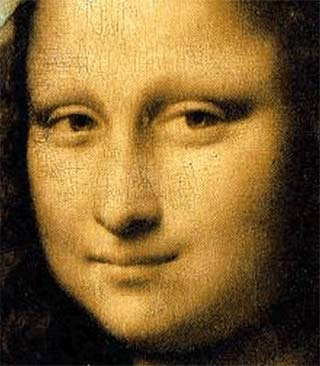
\includegraphics[height=4\baselineskip]{imgs/logo}\\ \vspace{0.2cm}
        \sffamily{\bfseries{ \Large \@subtitle}}\\
        \vspace{0.2cm}
        \sffamily{\bfseries{ \Huge \@title}}
        \vspace{0.6cm}
        \small \\
        A Bachelor Thesis presented to the Division of Computer Science\\ Department of Engineering and Information Technology, Bern University of Applied Sciences \\
        \vspace{0.1cm}
        Presented by \@author\\
        Supervised by Professor Olivier Biberstein, PhD\symbolfootnote[3]{\href{mailto:olivier.biberstein@bfh.ch}{olivier.biberstein@bfh.ch}}\\
        \vspace{0.2cm}
        \@date
        \vspace{0.5cm}
    \hrule
    \end{flushright}
		\vfill
    
\includegraphics[height=\baselineskip]{imgs/by-sa}\\ \small{\sffamily{Licensed under the Creative Commons Attribution-ShareAlike 3.0 License}}
    \end{titlepage}
}

%
% Headers and footers
%
\pagestyle{fancy}
\fancyhf{}

% no numbers for sections and chapters in headers
\renewcommand{\chaptermark}[1]{\markboth{#1}{}}
\renewcommand{\sectionmark}[1]{\markright{#1}{}}

\if@twoside
	% even pages footer
	\fancyfoot[EL]{\thepage}
	% odd pages footer
	\fancyfoot[OR]{\thepage}
	% even pages header
	\fancyhead[EC] {
			%chapter name
			\rightmark
	}
	\fancyhead[EL] {
			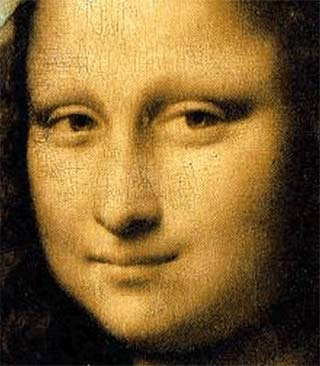
\includegraphics[height=2\baselineskip]{imgs/logo}
	}
	% odd pages header
	\fancyhead[OC] {
			%chapter name
			\leftmark
	}
	\fancyhead[OR]{
			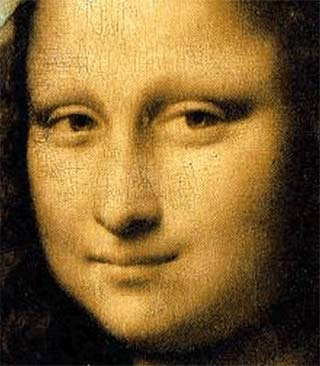
\includegraphics[height=2\baselineskip]{imgs/logo}
	}
\else
	\fancyfoot[C]{\thepage}
	\fancyhead[C] {
			%chapter name
			\rightmark
	}
	\fancyhead[R] {
			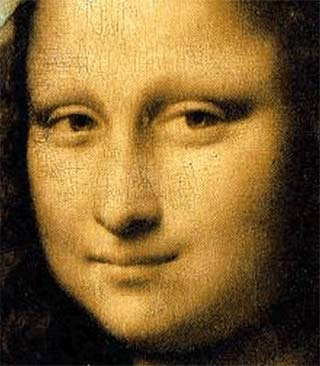
\includegraphics[height=2\baselineskip]{imgs/logo}
	}
\fi

% Table of content not contents
%\renewcommand\contentsname{Table of Contents}

%\addtolength{\headheight}{2\baselineskip}
%\addtolength{\headheight}{0.3pt}

%\renewcommand{\chaptermark}[1]{%
%\markboth{#1}{}}

%% second level list 1, 2, ...

\renewcommand{\labelenumii}{\arabic{enumii}.}

%%--------------------------------------------------------------------------
%% New environments and commands specific to this template.
%%--------------------------------------------------------------------------

%% special list for alternate scenario in usecase *a, *b, ...
\newenvironment{usecasealt}
    {
        \renewcommand{\labelenumi}{*\alph{enumi}.}
        \begin{enumerate}
    }
    {
        \end{enumerate}
        \renewcommand{\labelenumi}{\arabic{enumi})}
    }

\newenvironment{letterenum}
    {
        \renewcommand{\labelenumi}{\alph{enumi})}
        \begin{enumerate}
    }
    {
        \end{enumerate}
        \renewcommand{\labelenumi}{\arabic{enumi})}
    }
\newenvironment{numberenum}
    {
        \renewcommand{\labelenumi}{\arabic{enumi})}
        \begin{enumerate}
    }
    {
        \end{enumerate}
        \renewcommand{\labelenumi}{\alph{enumi})}
    }

%% Highlight for method names and other code source excerpt
\newcommand{\srcpart}[1]{{\fontfamily{cmtt}\selectfont #1}}

\newcommand{\image}[2]{
  \begin{figure}[htb]
      \centering
      \includegraphics{#1}
      \caption{#2}
  \end{figure}
}

\usepackage{amsthm}
\usepackage{ucs}
\usepackage{amsmath}
\usepackage{amsfonts}
\usepackage{amssymb}
\usepackage{emp}
\usepackage{xspace}

% 
% Some shortcuts
%
\usepackage{arev}
\newsavebox{\sharpbox}
\sbox{\sharpbox}{$\sharp$}
\def \cs {C\usebox{\sharpbox}\xspace}
\def \match {<\#\xspace}
\def \mytype {\emph{MyType}\xspace}
\def \ooplss {$\mathcal{OOPLSS}$\xspace}
\def \ra {$\rightarrow$\xspace}
\def \lra {$\longrightarrow$\xspace}


% switch back to Latin Modern
\usepackage{lmodern}

% this is apparently used for the metauml stuff
\ifx\pdftexversion\undefined
\usepackage[dvips]{graphicx}
\else
\usepackage{graphicx}
\DeclareGraphicsRule{*}{mps}{*}{}
\fi

\newtheorem{mydef}{Definition}

%
% TODO List
%
\ifx \showtodo \undefined
  \newcommand{\todo}[1]{}
	\newcommand{\listoftodos}{}
\else
	\newcommand{\todo}[1]{
	% Add to todo list
	\addcontentsline{tdo}{todo}{\protect{#1}}
	%
	\begin{tikzpicture}[remember picture, baseline=-0.75ex]
			\node [coordinate] (inText) {};
	\end{tikzpicture}
	%
	% Make the margin par
	\marginpar{
			\begin{tikzpicture}[remember picture]
					\definecolor{orange}{rgb}{1,0.5,0}
					\draw node[font=\footnotesize, draw=black, fill=orange, text width = 2.2cm] (inNote) {#1};
			\end{tikzpicture}
	}
	%
	\begin{tikzpicture}[remember picture, overlay,>=stealth]
			\draw[draw = orange, thick]
					([yshift=-0.2cm] inText)
							-| ([xshift=-0.2cm] inNote.west)
							-| (inNote.west);
	\end{tikzpicture}
	%
	}
	
	% TODO List
	\makeatletter \newcommand \listoftodos{\section*{Todo list} \@starttoc{tdo}}
		\newcommand\l@todo[2]
		{\par\noindent \textit{#2}, \parbox{10cm}{#1}\par} \makeatother
\fi

% journal itemize
\newenvironment{journal}%
  {\vspace{-0.45cm}
    \begin{itemize}%
      \setlength{\itemsep}{0pt}%
      \setlength{\parskip}{0pt}}%
  {\end{itemize}}

